\documentclass[border=1mm,
               class=article
               preview]{standalone}
\usepackage{tikz}
\begin{document}
\begin{tikzpicture}
    \node[anchor=south west,inner sep=0] (graph) at (0,0) {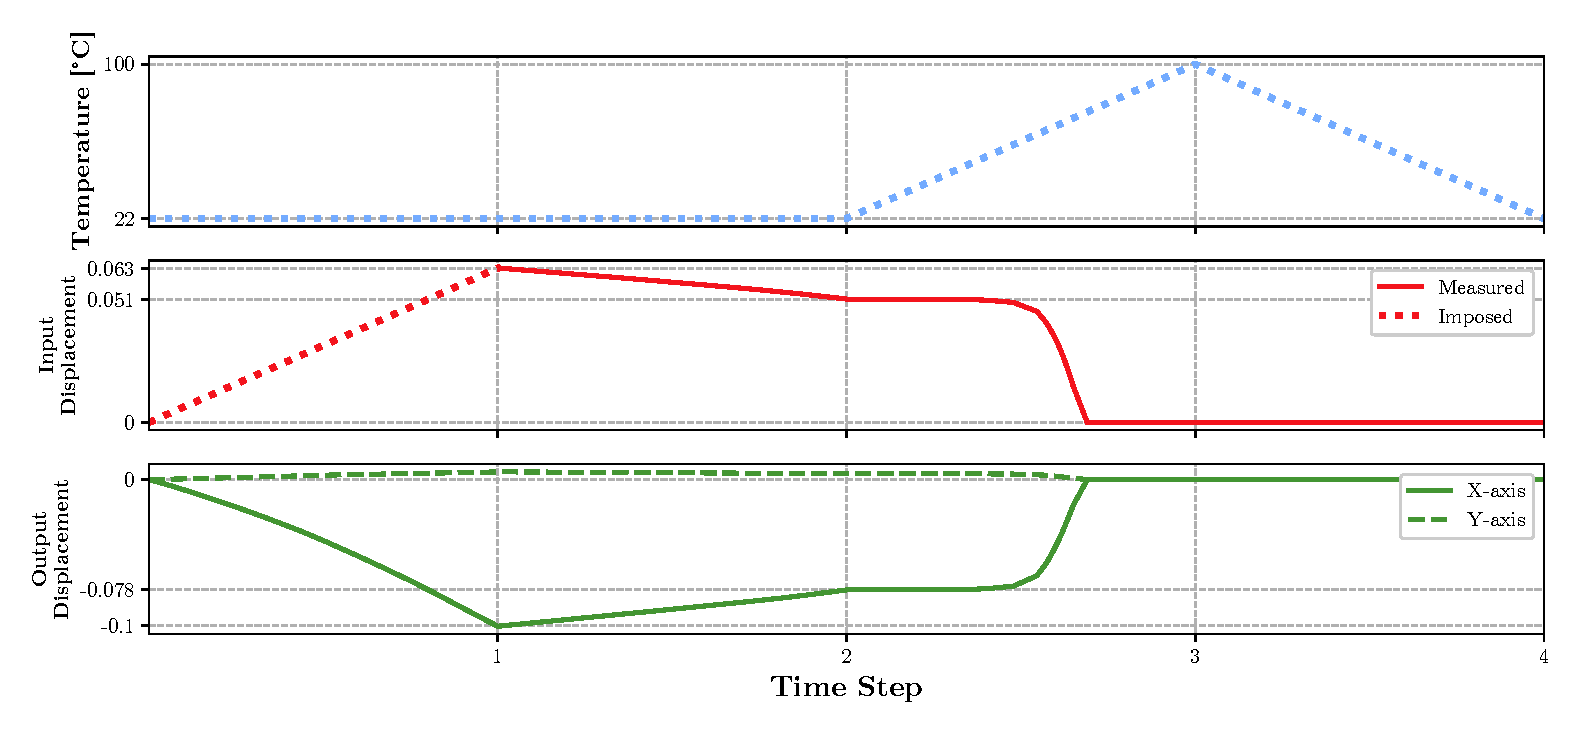
\includegraphics[width=\textwidth]{images/chap5/BM_Inverter30.eps}};
    \coordinate (ts0) at (1.54,7.6);
    \coordinate (ts4) at (17.55,7.6);
    \coordinate (ts1) at ($ (ts0)!0.25!(ts4) $);
    \coordinate (ts2) at ($ (ts0)!0.5!(ts4) $);
    \coordinate (ts3) at ($ (ts0)!0.75!(ts4) $);
    \node[anchor=mid,inner sep=0] (ls0) at ($(ts0)!0.5!(ts1) + (0,0.4) $) {\fbox{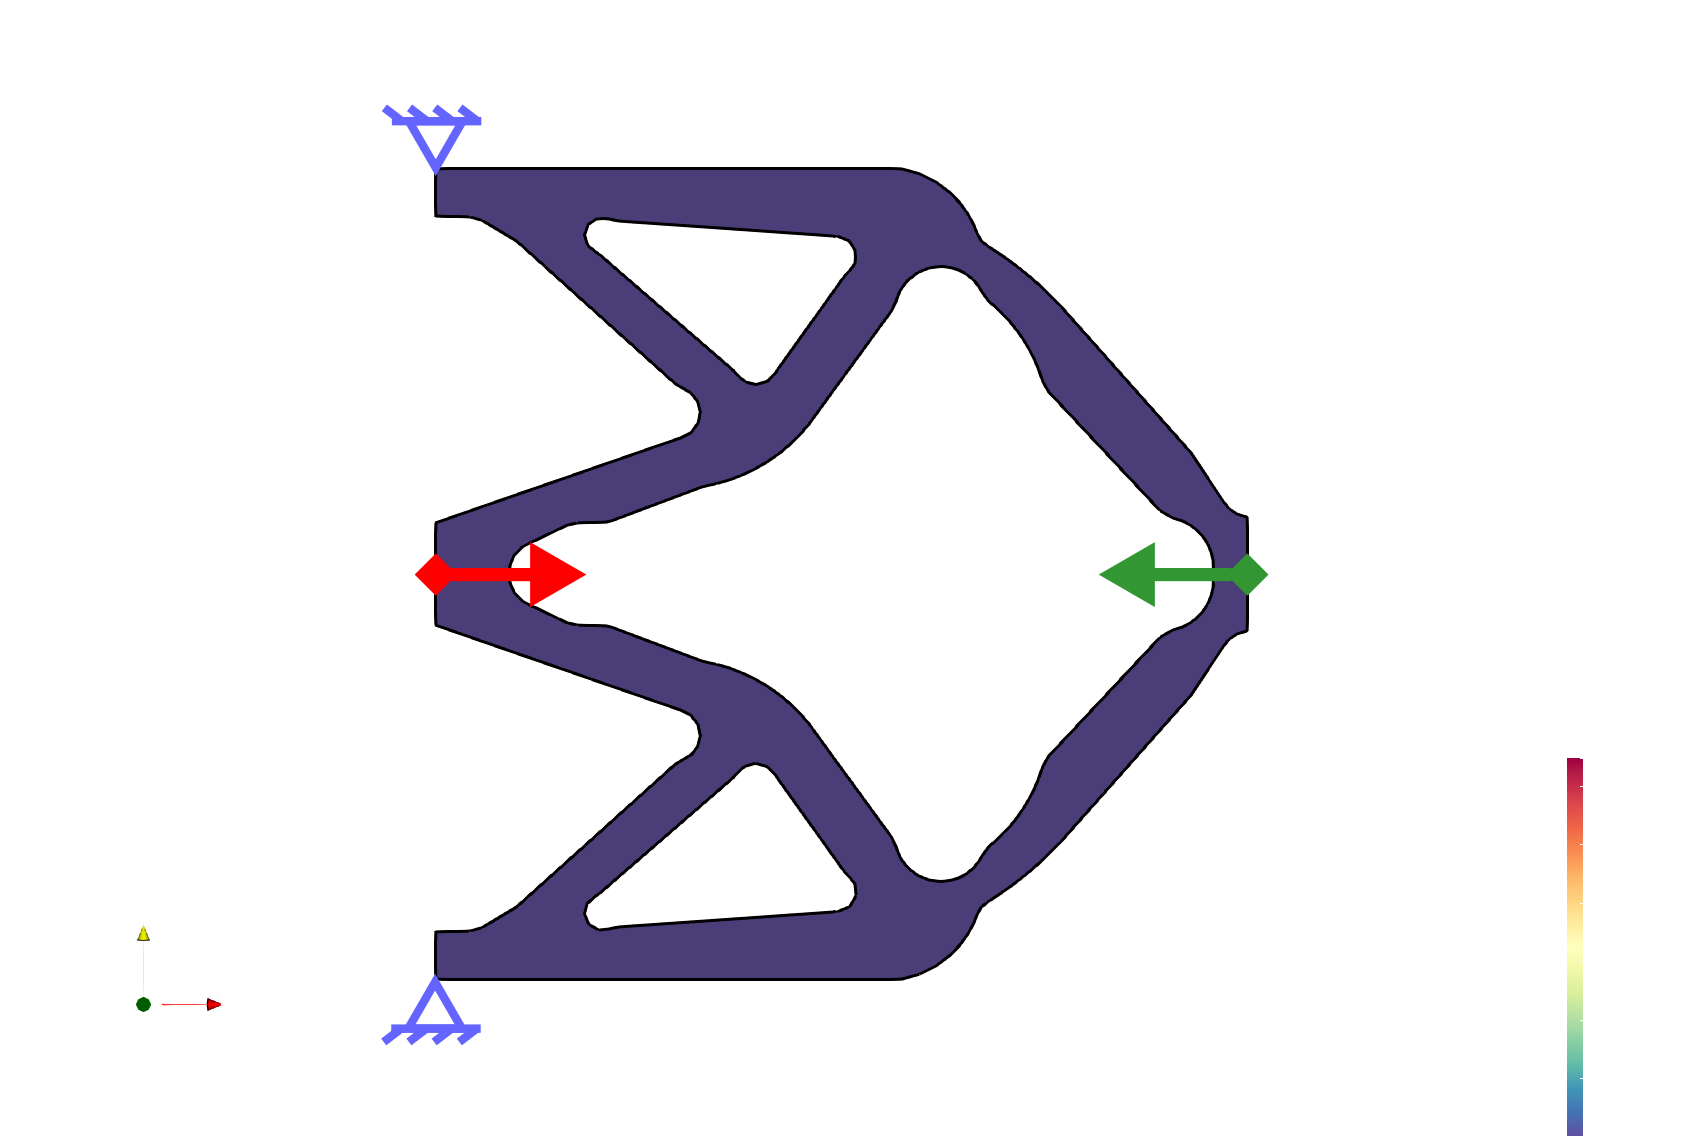
\includegraphics[height = 2cm,trim={11cm 3cm 13cm 3cm},clip]{images/chap5/Inverter_step0_v3.png}}};
    \draw[black, thick, -latex](ls0.west) to [bend right] (ts0);
    \node[anchor=mid,inner sep=0] (ls1) at ($(ts1)!0.5!(ts2) + (0,0.4) $) {\fbox{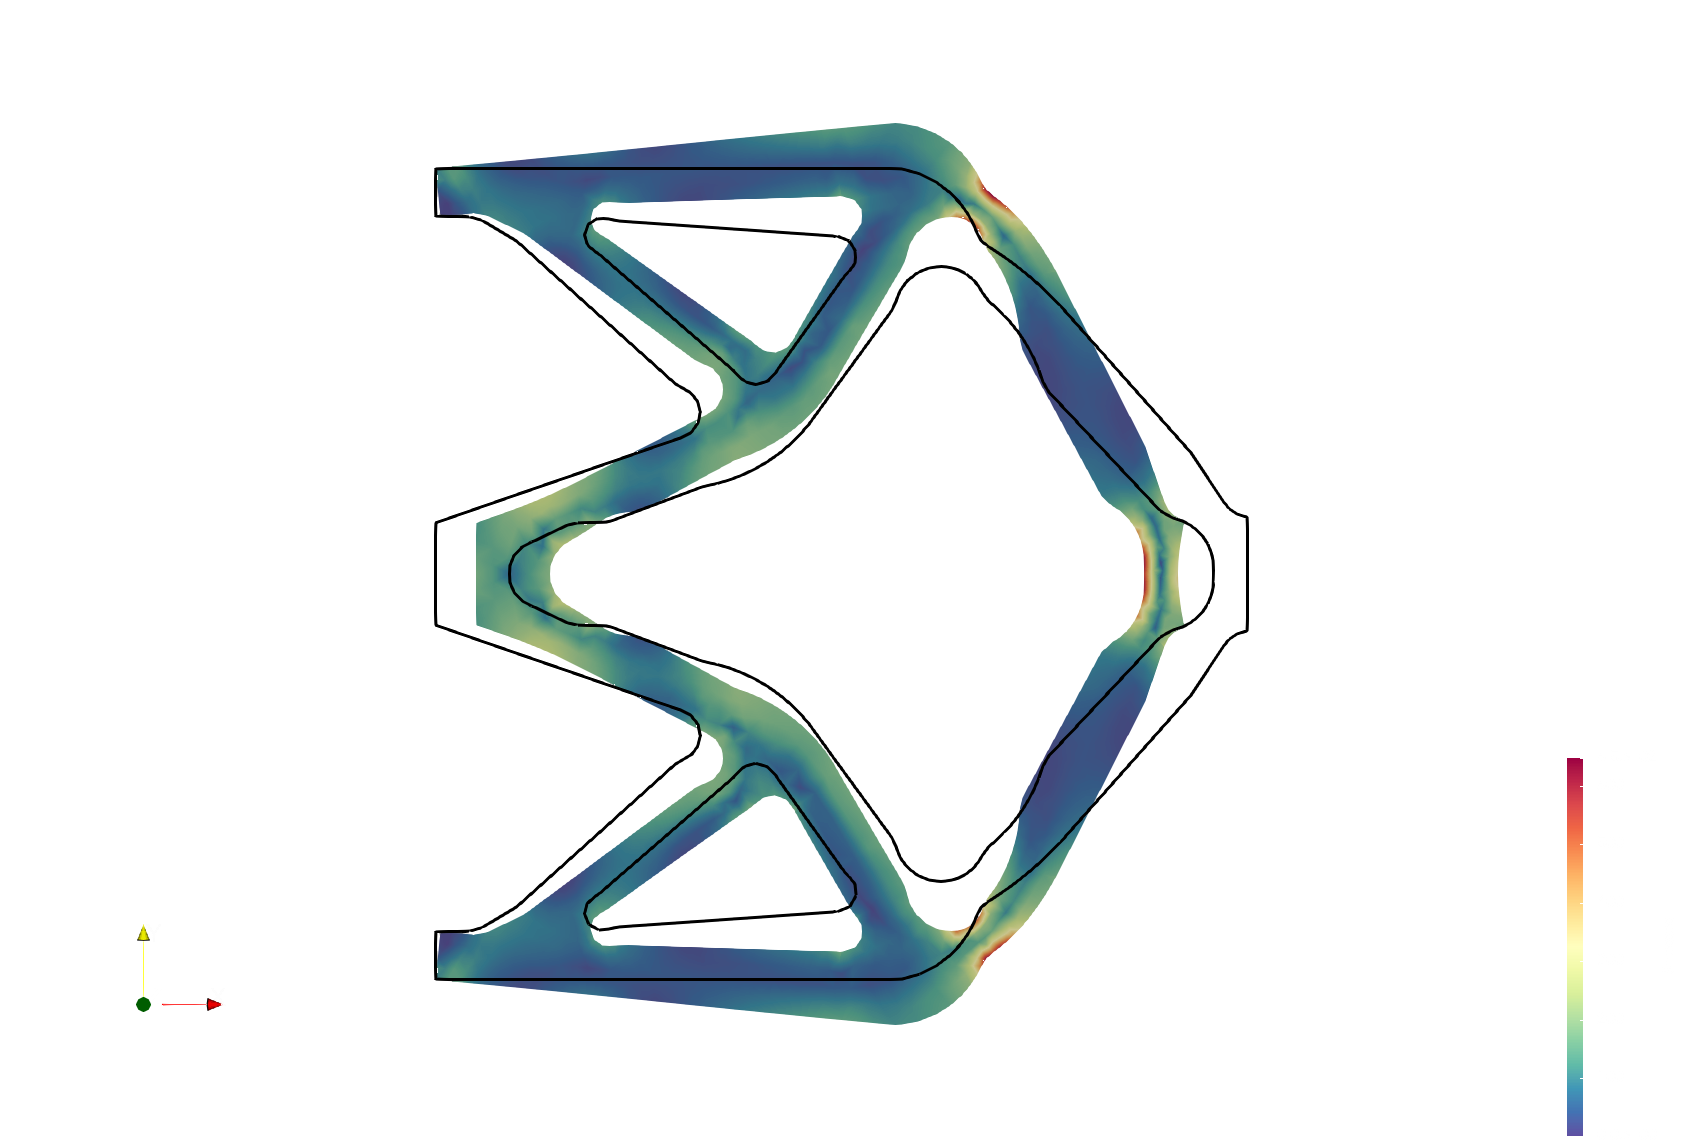
\includegraphics[height = 2cm,trim={11cm 3cm 13cm 3cm},clip]{images/chap5/Inverter_step1.png}}};
    \draw[black, thick, -latex](ls1.west) to [bend right] (ts1);
    \node[anchor=mid,inner sep=0] (ls2) at ($(ts2)!0.5!(ts3) + (0,0.4) $) {\fbox{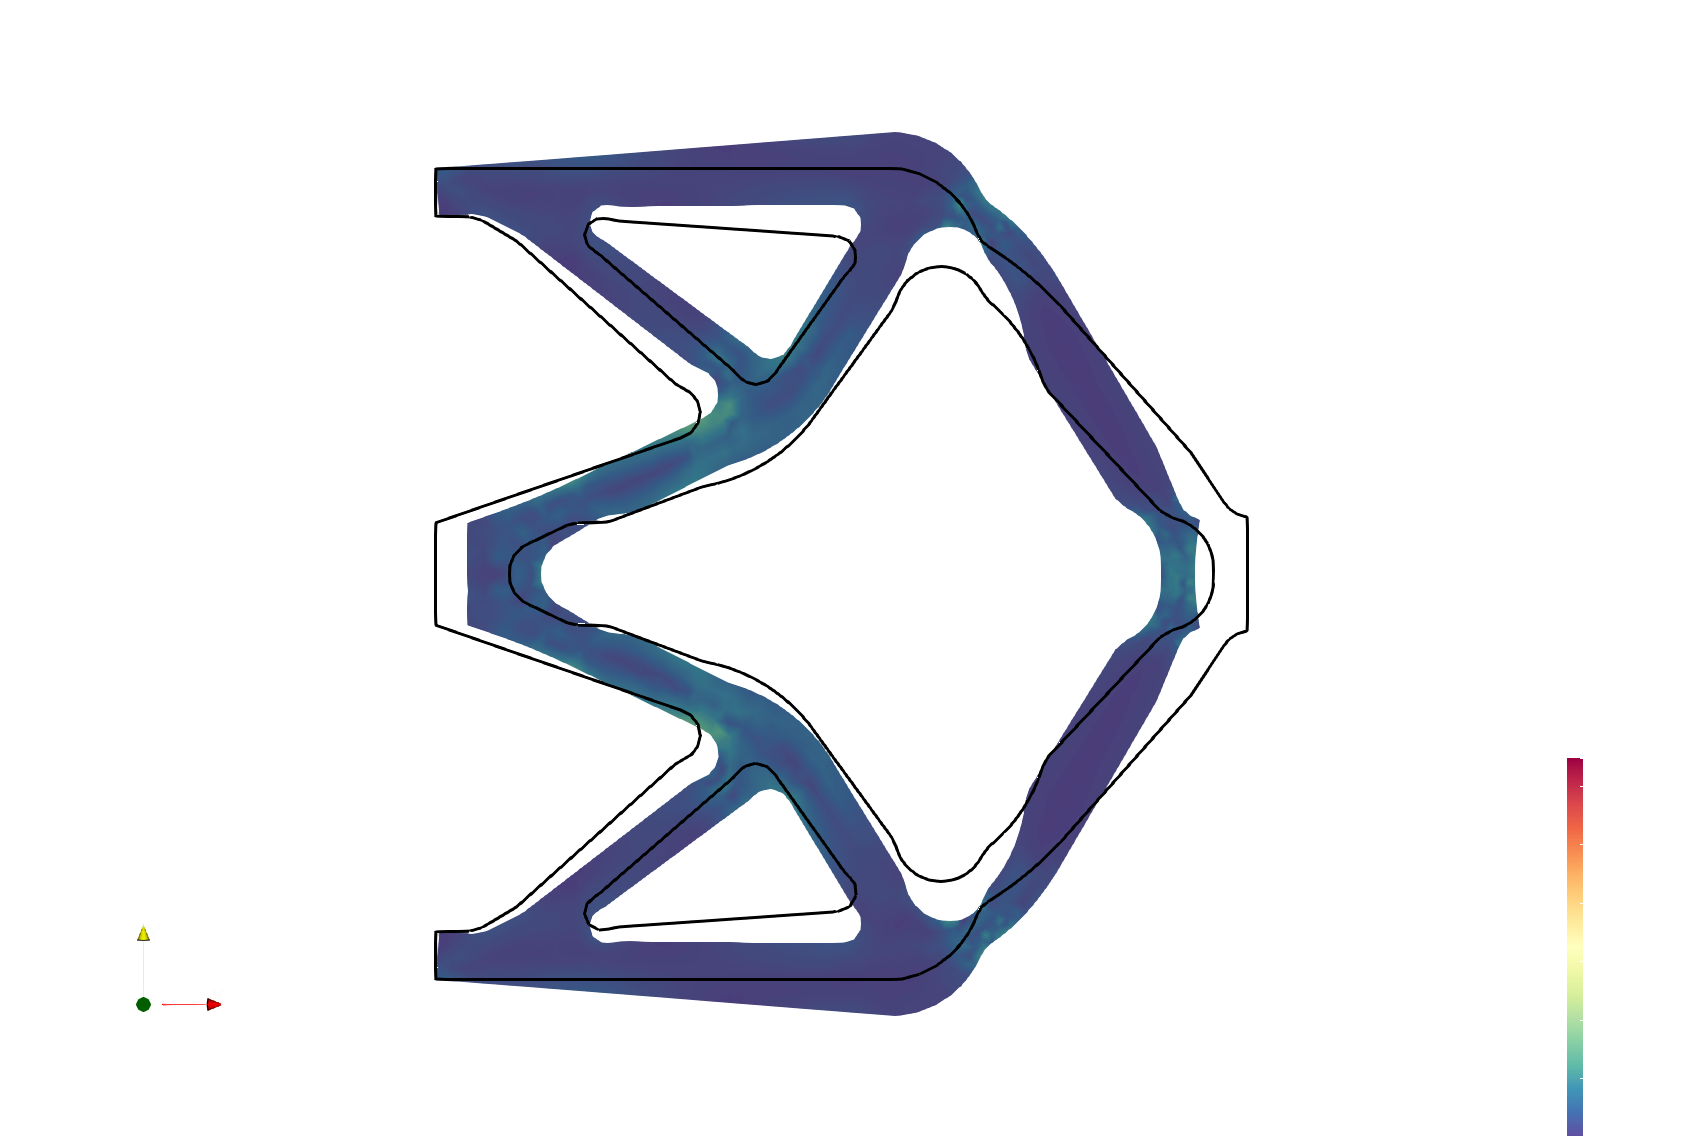
\includegraphics[height = 2cm,trim={11cm 3cm 13cm 3cm},clip]{images/chap5/Inverter_step2.png}}};
    \draw[black, thick, -latex](ls2.west) to [bend right] (ts2);
    \node[anchor=mid,inner sep=0] (ls3) at ($(ts3)!0.5!(ts4) + (0,0.4) $) {\fbox{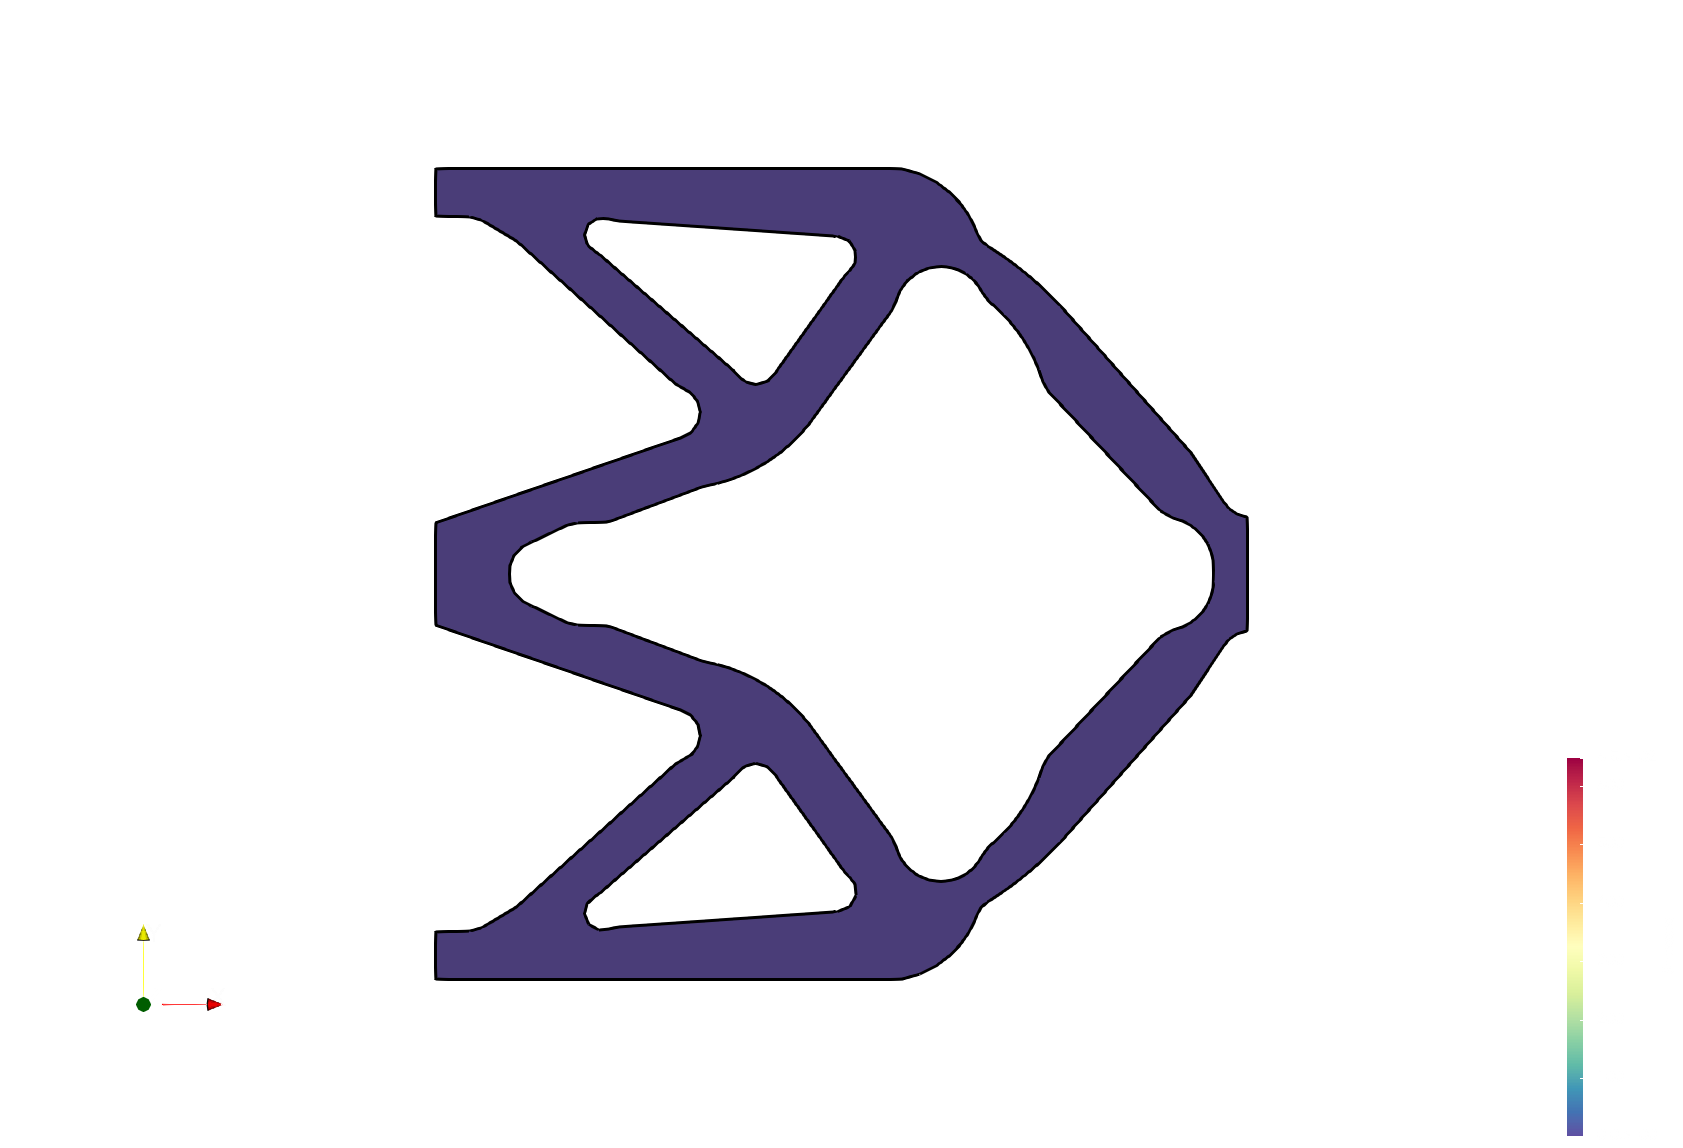
\includegraphics[height = 2cm,trim={11cm 3cm 13cm 3cm},clip]{images/chap5/Inverter_step0.png}}};
    \draw[black, thick, -latex](ls3.west) to [bend right] (ts3);
    \node[anchor=south east,inner sep=0] (ls0) at ($(ts4) + (0,0.15) $) {
\includegraphics[height = 2.3cm]{images/chap5/Colorbar.pdf}};
    \end{tikzpicture}%
\end{document}
